\documentclass[pdf]{beamer}
\mode<presentation>{\usecolortheme{crane}}
%% preamble
\title{Simulation of CSE Lab Cluster}
\subtitle{CS633 2018-19-II Course Project}
\author{Yash Srivastav (150839)}
\date{April 25, 2018}

% \AtBeginSection[]
% {
%   \begin{frame}{Table of Contents}
%     \tableofcontents[currentsection]
%   \end{frame}
% }

\AtBeginSubsection[]
{
  \begin{frame}{Table of Contents}
    \tableofcontents[currentsubsection]
  \end{frame}
}

\begin{document}
%% title frame
\begin{frame}
  \titlepage
\end{frame}
%% normal frame
\section{Introduction}
\subsection{Description}
\begin{frame}{CSE Lab Cluster}
  \begin{itemize}
    \item<1-> Consists of $\sim{} 30$ PCs connected over LAN
    \item<2-> Hostfiles used for MPI programs usually don't take topology or
      placement into account
    \item<3-> We want to simulate the running of an MPI program on this cluster
      and predict time taken for communications
    \item<4-> Would enable simulating under different hostfiles and use it to
      decide upon which one to use
  \end{itemize}
\end{frame}
\begin{frame}{CSE Lab Cluster Topology}
  \begin{figure}[ht]
    \begin{center}
      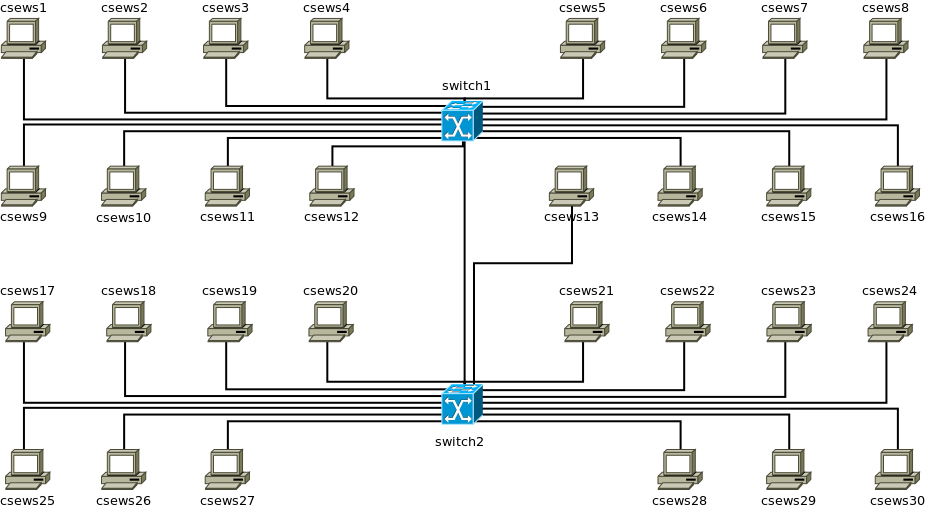
\includegraphics[width=\textwidth]{topology}
    \end{center}
  \end{figure}
  \begin{itemize}
    \item \texttt{csews13} is on different switch from remaining \texttt{csews1-16}
  \end{itemize}
\end{frame}
\subsection{Related Work}
\begin{frame}{Related Research Papers}
  \begin{itemize}
    \item MPI-NeTSim: A network simulation module for MPI \cite{netsim}
    \item Simulation of MPI Applications with Time-independent Traces
      \cite{time-independent-trace-sim}
    \item Single Node On-Line Simulation of MPI Applications with SMPI
      \cite{smpi-online}
    \item Toward Better Simulation of MPI Applications on Ethernet/TCP
      Networks \cite{better-sim-ethernet}
    \item Simulating MPI applications: the SMPI approach \cite{smpi}
  \end{itemize}
\end{frame}
\begin{frame}{Possible Approaches}
  \begin{itemize}
    \item<1-> Offline (post-mortem): Collect a trace of all functions being
      called and their arguments during a sample run. Use this trace to
      simulate any target run.
    \item<2-> Online (in-situ): Perform simulation while executing the program
      itself, usually by hooking into the network layer and redirecting network
      requests to a simulator.
    \item<3-> Hybrid: A combination of the above to have prior knowledge of the
      types of network communications supposed to happen and simulate better
      accordingly.
  \end{itemize}
\end{frame}
\begin{frame}{Salient points of previous papers}
  \begin{itemize}
    \item<1-> \cite{netsim} uses an online approach which hooks onto the MPI network
      layer and simulates it. Due to latency of simulation, the normal code itself
      has to be scaled to slow down. This may lead to slower simulations
    \item<2-> \cite{smpi} and \cite{smpi-online} use a complete reimplementation of
      the MPI specification on the \textbf{SimGrid} simulation kernek with a
      hybrid approach. Hence its not possible to switch out one MPI implementation
      for another.
    \item<3-> Even \cite{time-independent-trace-sim} uses the above smpi
      implementation even though it is an offline approach
  \end{itemize}
\end{frame}
\subsection{Approach and Challenges}
\begin{frame}{Approach}
  \begin{itemize}
    \item<1-> Obtain time-independent event traces for the target MPI program
      similar to \cite{time-independent-trace-sim}.
    \item<2-> The above gives us bytes transferred and to whom (for
      communications) and number of instructions executed (for computations).
    \item<3-> Using the knowledge of the network topology and a given hostfile,
      perform simulation based on the trace obtained on \textbf{ns3}.
    \item<4-> Report the expected time taken.
  \end{itemize}
\end{frame}
\begin{frame}{Obtaining Event Traces}
  \begin{itemize}
    \item<1-> We use the \texttt{PMPI\_} interface exposed by nearly all MPI
      implementations inorder to override calls to \texttt{MPI\_} functions with
      custom code. This allows us to trace calls to those functions.
    \item<2-> We also use the \textbf{Performance Application Programming
        Interface (PAPI)} \cite{papi} in order to measure CPU cycles /
      instructions between 2 MPI calls (computation). Since PAPI counters are
      thread specific, this approach is valid on over-subscribed MPI executions
      as well.
    \item<3-> At the end of an invocation of an MPI call, we note down the value
      of the performance counter. At the start of the next MPI call, the
      difference between the counter value are the computation instructions.
  \end{itemize}
  % Challenges:
\end{frame}
\begin{frame}{Obtaining Event Traces - Challenges / Drawbacks}
  \begin{itemize}
    \item<1-> In order to collect the traces on a single machine, the machine
      should have enough memory for all the processes.
    \item<2-> The trace size grows pretty large for non-trivial applications.
    \item<3-> The tracing machine should have the same processor architecture
      as the CSE lab cluster. Since our tracer would run on one of the lab
      machines, it is not an issue.
  \end{itemize}
\end{frame}
\begin{frame}{Offline Simulation}
  \begin{itemize}
    \item<1-> Using the information collected by the traces and a provided
      hostfile, we could generate an event stream for each node on the cluster.
    \item<2-> The above event stream would be fed into an event-based network
      simulator like ns3 which has all the hosts configured as per the cse lab
      cluster topology.
    \item<3-> This should give us the expected time for each event.
  \end{itemize}
\end{frame}
\section{Features and Implementation}
\subsection{Features}
\begin{frame}{MPI Calls}
  The simulator simulates/handles the following synchronous MPI calls with
  algorithms as used in default \texttt{MPICH v3.2.1}:
  \begin{itemize}
    \item \texttt{MPI\_Send}
    \item \texttt{MPI\_Recv}
    \item \texttt{MPI\_Scatter}
    \item \texttt{MPI\_Gather}
    \item \texttt{MPI\_Broadcast} (only the algorithm for short messages for
      now)
  \end{itemize}
\end{frame}
\begin{frame}[fragile]
  \frametitle{Simulation Semantics (tracing)}
  This is how the \textbf{Sim}ulated \textbf{MPI} tracer is used:
  \begin{semiverbatim}
    \$ export LD\_PRELOAD=libpapi.so:libsimpi.so
    \$ mpirun -np 32 prog.x
    \$ cat *.log
  \end{semiverbatim}
  This gives us a trace/log of all MPI function calls we are interested in.
\end{frame}
\begin{frame}[fragile]
  \frametitle{Simulation Semantics (simulation)}
  This is how the simulator is invoked:
  \begin{semiverbatim}
    \$ ./run-simulator.sh 64 hostfile path/to/log
  \end{semiverbatim}
  This gives us a value for the expected simulation time.
\end{frame}

\subsection{Implementation}

\begin{frame}{Tracer}
  \begin{itemize}
    \item<1-> A compiled static library which can be used with
      \texttt{LD\_PRELOAD}
    \item<2-> Logs all relevant info of an MPI function call whenever it is
      encountered.
    \item<3-> Each MPI process opens up a log file during \texttt{MPI\_Init} and
      closes it during \texttt{MPI\_Finalize}.
  \end{itemize}
\end{frame}
\begin{frame}{Simulator}
  \begin{itemize}
    \item<1-> Consists of 3 major components: the parser, topology generator and
      the main \texttt{MPINode} \texttt{ns3::Application}.
    \item<2-> The parser parses the given log files to generate event log for
      every process
    \item<3-> The topology generator sets up the entire network as per the CSE
      lab cluster.
    \item<4-> \texttt{MPINode} is an \texttt{ns3::Application} supposed to
      behave like our MPI process. An \texttt{ns3::Application} can be installed
      on any node on the network. We install 1 MPI application corresponding to
      each MPI process. So there are PPN number of applications running on a
      node.
  \end{itemize}
\end{frame}
\begin{frame}{Parser}
  \begin{itemize}
    \item<1-> Parses event logs to an event stream which can be simulated by
      \texttt{MPINode}.
    \item<2-> Event stream consists of only the following types of events:
      \texttt{Compute}, \texttt{Recv} \& \texttt{Send}.
    \item<3-> Any other kind of event like \texttt{MPI\_Scatter} is converted
      into a mixture of the above events as per the communications taking place
      according to the algorithms.
  \end{itemize}
\end{frame}
\begin{frame}{\texttt{MPINode}}
  \begin{itemize}
    \item<1-> Essentially a tcp server + client.
    \item<2-> Events are processed sequentially as soon as the previous one
      finishes. Once there are no more events left, the application is
      stopped. Once all applications stop we can claim that the simulation has
      ended.
    \item<3-> For compute events, an artificial delay is introduced.
    \item<4-> For send and receive, normal socket operations are used.
  \end{itemize}
\end{frame}

\subsection{Demo}
\begin{frame}[c]
  \begin{center}
    \Huge Demo
  \end{center}
\end{frame}

\subsection{Future Possibilities}
\begin{frame}{Future Possibilities}
  \begin{itemize}
    \item<1-> Add support for different communicators.
    \item<2-> Add support for handling \texttt{MPI} function errors during
      tracing and logging them as well for use during simulation.
    \item<3-> Remaining collectives and Async variants of \texttt{MPI} functions and
      associated calls like \texttt{MPI\_Wait}
    \item<4-> Vector variants of \texttt{MPI} collectives (like
      \texttt{MPI\_Allgatherv})
    \item<5-> Allow greater send and receive sizes (fix socket + packet sending
      issue).
    \item<6-> Comparison with other \texttt{MPI} simulation frameworks developed as
      part of other works.
    \item<7-> Distributed trace collection: The trace collection itself could be run
      parallelly on multiple machines for faster trace collection and simulation.
  \end{itemize}
\end{frame}
\section{Conclusion}
\begin{frame}[c]
  \begin{center}
    \Huge Thank You!\\ \vspace{2mm}
    \tiny ``So long and thanks for all the fish.''  -- Douglas Adams
  \end{center}
\end{frame}
\subsection{References}
\begin{frame}[allowframebreaks]
  \frametitle{References}
  \bibliographystyle{IEEEtran}
  \bibliography{paper}
\end{frame}

\end{document}
